\documentclass{article}[a4paper,12pt]
\usepackage[utf8]{inputenc}
\usepackage{amsmath,amssymb,amsthm,amsfonts,mathtools}
\usepackage[inline]{enumitem}
\usepackage{soul}
\usepackage{cancel}
\usepackage{hyperref}
\usepackage{centernot}
\usepackage{pifont}
\usepackage{changepage}
\usepackage{subcaption}
\usepackage[section]{placeins}
\usepackage{lipsum, graphicx, caption}
\usepackage{float}
\usepackage{commath}
\usepackage{wrapfig}
\usepackage{amsmath}
\usepackage{amsfonts}
\usepackage{amssymb}
\theoremstyle{definition}
\newtheorem{innercustomgeneric}{\customgenericname}
\providecommand{\customgenericname}{}
\newcommand{\newcustomtheorem}[2]{%
  \newenvironment{#1}[1]
  {%
   \renewcommand\customgenericname{#2}%
   \renewcommand\theinnercustomgeneric{##1}%
   \innercustomgeneric
  }
  {\endinnercustomgeneric}
}
\newcustomtheorem{customthm}{Theorem}
\newcustomtheorem{customlem}{Lemma}
\newcustomtheorem{customdefn}{Definition}
\newcustomtheorem{customprop}{Proposition}
\newcustomtheorem{customexer}{Exercise}
\renewcommand{\qedsymbol}{$\blacksquare$}

\newcommand{\Lagr}{\mathcal{L}}

\setlength\parindent{0pt}
\let\emptyset\varnothing
\usepackage{geometry}
\geometry{
	a4paper, portrait,
	total = {170mm,257mm},
	left = 20mm,
	top = 20mm,
}

\usepackage{xcolor}
\usepackage{pagecolor}
\pagecolor{white}
\color{black}

\title{\textbf{Neural Networks and Deep Learning}}
\author{
	\textbf{Om Prabhu}\\
	19D170018\\
	Undergraduate, Department of Energy Science and Engineering\\
	Indian Institute of Technology Bombay\\}
\date{Last updated \today}

\begin{document}
\maketitle
\vspace{-12pt}
\hrulefill
\vspace{6pt}

\textbf{NOTE:} This document is a brief compilation of my notes taken during the course `Neural Networks and Deep Learning'. You are free to use it and my project files for your own personal use \& modification. You may check out the course and/or specialization here: \texttt{\href{https://www.deeplearning.ai/}{deeplearning.ai}}.

\hrulefill
\tableofcontents
\vspace{6pt}

\hrulefill
\pagebreak

\section{Introduction}
\subsection{About myself}
Hello. I am Om Prabhu, currently an undergrad at the Department of Energy Science and Engineering, IIT Bombay. If you have gone through my website (\texttt{\href{https://omprabhu31.github.io/}{https://omprabhu31.github.io/}}) earlier, which is probably where you found this document too, you will know that I am quite a bit into programming and tinkering with code to try and do cool stuff. Additionally, I love playing video games, listening to music and engaging in a little bit of creative writing as and when I get time. With this brief self-introduction, let us get into why I decided to pursue this course.
\subsection{A little bit about deep learning}
As you probably know, deep learning has already transformed traditional internet businesses like web search and advertising. Further, it is also helping in the creation of businesses and business products and even jobs. Deep learning is making it into almost all types of industries ranging from healthcare and medical diagnosis to personalized education, precision agriculture and many others. 
\vspace{6pt}

Just as how electricity once transformed countless industries, AI today is on its way to doing the same. The part of AI that is contributing to most of this transformation is deep learning. This is a technical course which will teach us how to build neural networks and by the end of this course, we will be able to build a cat recognizer (for some reason, there is this cat meme running around in the world of AI which will also be discussed later).

\hrulefill
\pagebreak
\section{Overview of Deep Learning}
The terminology in AI is still not very well defined. For example, some people say that neural networks are a subset of deep learning while others use the two words almost interchangeably. Through most of this documentation, we will refer to deep learning as being a science of building and training neural networks. With that said, let's look at what a neural network is.
\subsection{Neural networks}
Let us use an example of demand prediction to try and understand what neural networks really are. Suppose a t-shirt company wants to know how many units they can expect to sell based on their selling price. The required dataset might be a in the form of a demand curve, where the higher the price the lesser the demand. This form of curve can be used to train what is perhaps the simplest possible neural network.
\begin{center}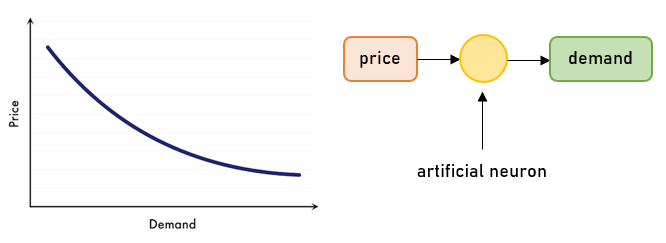
\includegraphics{deep_learning1.png}\end{center}
All this single-neuron network does is compute the curve shown and `learn' it in order to map any value of price to the appropriate value of demand. A single neuron can be thought of as a Lego brick, and a neural network as a very complicated stack, often in multiple layers, of such bricks.
\vspace{6pt}

Let's look at a more complicated example. Suppose that instead of just the price, we have more variables like shipping cost, marketing cost and material. Then we will have multiple factors that influence demand like affordability, consumer awareness and perceived quality. We might then have a slightly more complicated neural net like the one below:
\begin{center}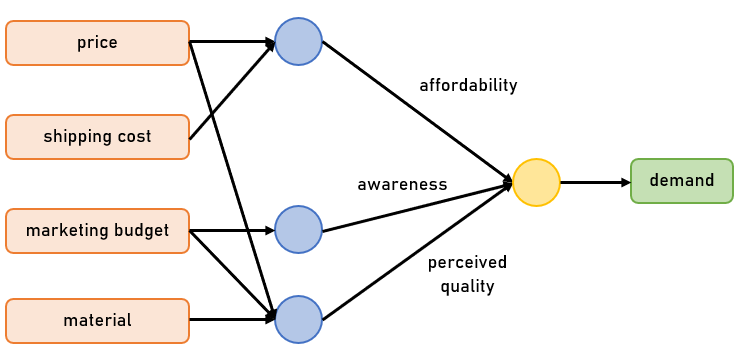
\includegraphics{deep_learning2.png}\end{center}
This slightly more complicated neural network maps the 4 input parameters to the output that is the demand.
\vspace{6pt}

From that the way in which we have discussed neural networks above, it appears as if we have to actually figure out the key factors as affordability, awareness and perceived quality. However, things do not work this way. One of the best things about neural networks is that we only have to provide it the input and the output $-$ all of the stuff in the middle, it figures out by itself. It automatically `learns' and completely trains itself to find the most accurate possible function that maps from the input to the output.
\vspace{6pt}

Another little correction is that it seems like the first node takes in only price and shipping inputs and so on. This is not the case. In practice, all nodes will be fed in with all the inputs and we let the individual neurons decide how many inputs they want to use and how they use them.
\subsection{Supervised learning with neural networks}
Most of the value created through deep learning has been in applications of supervised learning. This is the task of learning a function that maps an input to an output based on example input-output pairs (or A $\rightarrow$ B mapping). This has turned out to be very profitable for many industries such as:
\begin{itemize}
	\item online advertising: input is ad \& user info using which the algorithm tries to figure out if the user is likely to click on the ad
	\item computer vision: this is a very vast application area of AI (for example, input is an image and the algorithm tries to figure out whether the image is part of a dataset of 1000 images)
	\item speech recognition: input an audio clip and output a text transcript based on the input
	\item machine translation: input text or documents in certain languages and receive a translated output
	\item autonomous driving: AI algorithm uses image \& sensor info to figure out the position of nearby cars so it can avoid them
\end{itemize}
It turns out that slightly different types of neural networks are useful for different applications. For example, convolutional neural networks (CNN) are most commonly used for image applications while recurrent neural networks (RNN) are better for processing sequential data such as audio. More complicated applications often require the generation of custom neural network architecture.
\begin{center}
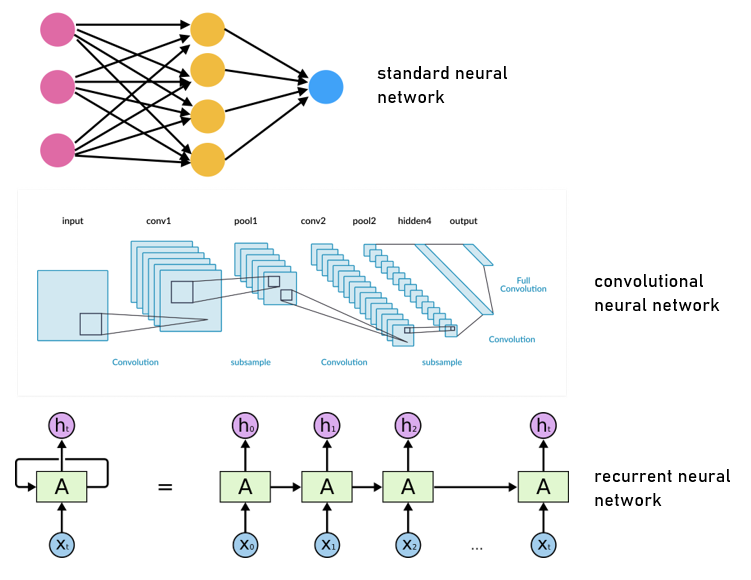
\includegraphics{types_of_nn.png}
\end{center}
Finally, supervised learning can be applied to both structured data (highly organized data such as tables, spreadsheets and databases) as well as unstructured data (data in the form of images, audio, video and even raw text).
\subsection{Why is deep learning taking off now?}
The ideas for deep learning and neural networks have been around for decades. Why is it that they have taken off only recently?
\vspace{6pt}

One of the major drivers of deep learning is scale. This refers to the ability of technology to train large sets of neural networks to process huge amounts of data while also improving AI performance. This can be illustrated through a graph as follows:
\begin{center}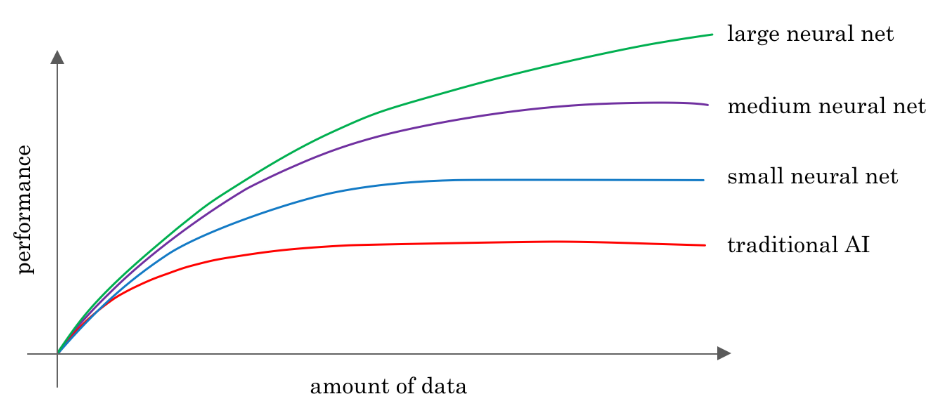
\includegraphics[scale=0.65]{data_vs_performance.png}\end{center}
\begin{itemize}
	\item for traditional deep learning systems, the data vs performance graph maxes out pretty early
	\item on training increasingly complex neural networks with higher amounts of data, performance keeps on getting better for much longer  
\end{itemize}
Hence to achieve the highest performance levels, we need two things. Firstly, it helps to have a lot of data. Additionally, we need the ability to train large sets of neural networks. Earlier, it was almost as if AI systems didn't know what to do with huge amounts of data. Now, with fast \& powerful CPUs and GPUs, it is possible for us to train large neural networks with a high amount of data.
\vspace{6pt}

Another factor is that of algorithmic innovation in order to increase the training speeds of neural networks. One of the major breakthroughs in this area has been the switch from sigmoid functions to ReLU functions:
\begin{center}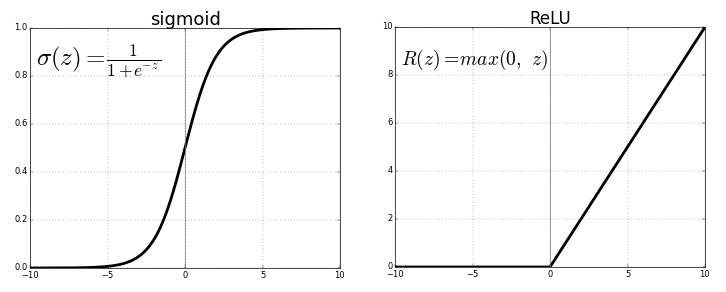
\includegraphics[scale=0.5]{sigmoid_relu.png}\end{center}
It turns out that on the tapering ends of the sigmoid function, since the gradient is nearly zero, the parameters hardly change and the training becomes very slow. In a ReLU curve, the gradient does not gradually shift to zero, so there is no point where the learning speed of the network is very slow. 
\vspace{6pt}

Fast computation is very important in deep learning, since the idea of training a neural network involves a lot of iterating $-$ basically we input the data, then train the neural network, then get feedback about how well the neural network performed, and then make changes to the data and neural network and repeat the cycle over and over until the neural network is trained well enough. Hence by reducing computation speeds, it leads to a huge rise in productivity while building out neural networks for AI projects.

\hrulefill
\begin{center}\textbf{END OF WEEK 1}\end{center}
This is the end of the course documentation from Week 1. Keep on reading further for documentation from further weeks, or spend some time gaining further insight into the previously discussed topics.

\hrulefill
\pagebreak
\section{Logistic Regression as a Neural Network}
Now that we have an idea of what neural networks are and what they can do, let us dive into the basics of neural network programming. Many of these ideas can be discussed using the concept of logistic regression.
\vspace{6pt}

\textbf{NOTE:} Throughout this section and some other parts of the document, there will be extensive use of the following notation:
\begin{enumerate}
	\item a single input feature vector has dimension $n_x$
	\item a single training example is represented by $(x,y)$ $\rightarrow$ $x\in\mathbb{R}^{n_x},$ $y\in\{0,1\}$
	\item a training set comprises $m$ (or $m_{train}$) training examples, i.e. $\{(x^{(1)},y^{(1)}), (x^{(2)},y^{(2)}), \dots, (x^{(m)},y^{(m)})\}$
	\item a test set similarly contains $m$ (or $m_{test}$) test examples
	\item to put all training examples $x$ into a more compact notation, we define a matrix $X\in\mathbb{R}^{n_x\times m}$ as follows:
\begin{center}
$X$ = 
$\begin{pmatrix}
	\vdots & \vdots & & \vdots\\
	x^{(1)} & x^{(2)} & \cdots & x^{(m)}\\
	\vdots & \vdots & & \vdots\\
\end{pmatrix}$
\end{center}
	\item to put all output labels $y$ into a more compact notation, we define a matrix $Y\in\mathbb{R}^{1\times m}$ as follows:
\begin{center}
$Y$ = 
$\begin{pmatrix}
	y^{(1)} & y^{(2)} & \cdots & y^{(m)}\\
\end{pmatrix}$
\end{center}
	\item terms of the form $x^{(i)}$, $y^{(i)}$, etc are associated with the $i^{th}$ training example
\end{enumerate}
\subsection{Derivatives (optional)}
Throughout this document, there will be a lot of differential calculus (i.e. the calculus of derivatives). Let us get somewhat familiar with derivatives before we move on to other concepts. This is by no means a comprehensive guide on differential calculus, for which you may look through some of the resources at the end of this section.

\begin{wrapfigure}[13]{L}{0.3\textwidth}
\centering 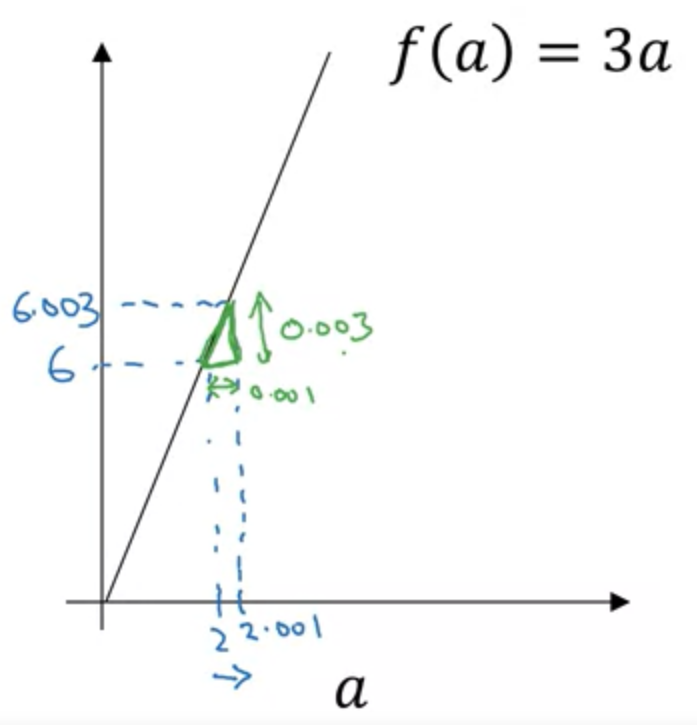
\includegraphics[width=0.28\textwidth]{y_equals_3x.png}
\end{wrapfigure}
\vspace{6pt}

Consider this simple function $f(a)=3a$. Let $a=2$, then $f(a)=6$. Let's now change $a$ by a very small amount, maybe $a=2.001$. Then we get $f(a)=6.003$.
\vspace{6pt}

Now if we construct a triangle as in the diagram, we see that `nudging' $a$ to the right by $0.001$ causes $f(a)$ to increase by $0.003$. For each 1 unit of change in $a$, there is a corresponding change of 3 units in $f(a)$. 
\vspace{6pt}

We say that the slope, or derivative, of the function $f(a)$ is 3. More specifically, it is the derivative of the function at $a=2$. More formally, we define the derivative of a function at a specific point as the rate of change of the function value at that point. Mathematically, we can write this as
$$\frac{\text{d}f(a)}{\text{d}a}=3=f^{\prime}(a)$$

\begin{wrapfigure}[10]{R}{0.31\textwidth}
\centering 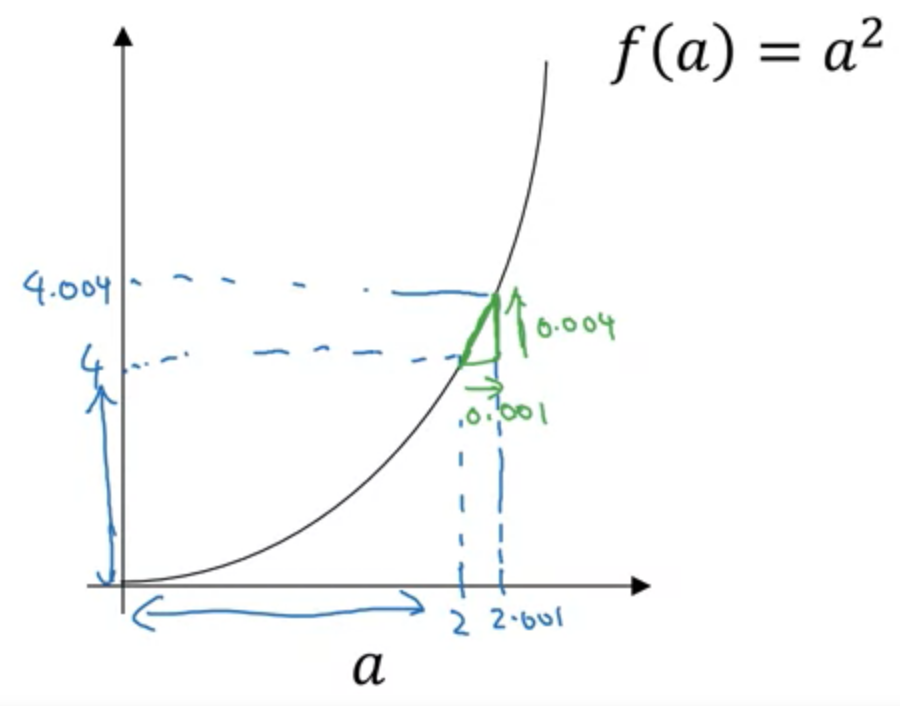
\includegraphics[width=0.31\textwidth]{x_square.png}
\end{wrapfigure}
\vspace{6pt}

The function represented above is a typical linear function $-$ its derivative at any point along the function is constant. Let us take a more complicated example, $f(a)=a^2$. At $a=2$, $f(a)=4$. Now, on changing $a=2.001$, we get $f(a)=4.004001\approx4.004$. 
\vspace{6pt}

Constructing a similar triangle, we can conclude that the slope of the function at $a=2$ is 4. What about at $a=5$?
\vspace{6pt}

At $a=5$, $f(a)=25$ while at $a=5.001$, $f(a)=25.010001\approx 25.01$. Again by a quick computation, the slope of the function at $a=5$ comes out to be 10.
\vspace{6pt}

As it happens, the derivative of the function $f(a)=a^2$ at any given point on the function is $2a$. 

\vspace{6pt}

This description of derivatives might make it look like they are an approximation, but this is not the case. In practice, the amount by which $a$ is changed is infinitesimally small, which gives rise to another concept in calculus known as limits (will not be discussed here). 
\pagebreak

If you wish to know more about derivatives and/or limits, feel free to go through the resources listed below: 
\begin{itemize}
	\item \texttt{\href{https://www.khanacademy.org/math/calculus-1/cs1-limits-and-continuity}{Limits and Continuity (by Khan Academy)}}
	\item \texttt{\href{https://www.khanacademy.org/math/calculus-1/cs1-derivatives-definition-and-basic-rules}{Derivatives: Definition and Basic Rules (by Khan Academy)}}
	\item \texttt{\href{https://www.khanacademy.org/math/calculus-1/cs1-derivatives-chain-rule-and-other-advanced-topics}{Derivatives: Chain Rule and Other Advanced Topics (by Khan Academy)}}
	\item \texttt{\href{https://www.khanacademy.org/math/calculus-1/cs1-applications-of-derivatives}{Application of Derivatives (by Khan Academy)}}
	\item \texttt{\href{http://www-math.mit.edu/~djk/calculus_beginners/}{Calculus for Beginners - MIT Mathematics}}
	\item \texttt{\href{https://ocw.mit.edu/resources/res-18-001-calculus-online-textbook-spring-2005/textbook/}{Online Calculus Textbook - MIT OpenCourseWare}}
	\item \texttt{\href{https://math.stackexchange.com/questions/tagged/calculus}{Mathematics StackExchange - Tags (Calculus)}}
\end{itemize}

\subsection{Binary classification}
Logistic regression is an algorithm for binary classification. An example of binary classification is taking in an input of an image and classifying it as a cat or not a cat. Let's look at how images are represented in computers.
\vspace{6pt}

Humans perceive images by their subtle features. A computer looks at an image as an array of pixels. A computer stores 3 separate matrices, each the size of the pixel map (i.e. 1920$\times$1080, 1024$\times$768, etc), corresponding to the RGB channels of the image. To process images, a computer `unpacks' the pixel intensity values to create what is known as a feature vector. 

\begin{wrapfigure}[7]{L}{0.5\textwidth}
\centering 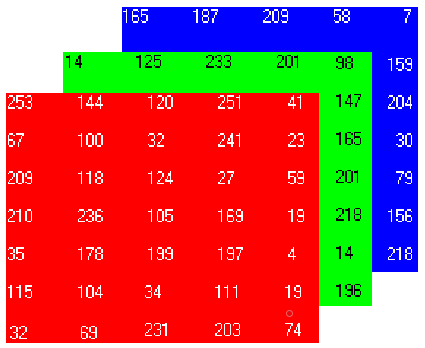
\includegraphics[width=0.48\textwidth]{rgb_matrices.png}
\end{wrapfigure}

We just take all the red pixel values and list them one by one, followed by the green pixel values and then the blue pixel values, as shown below:
\begin{center}
$x$ =
$\begin{pmatrix}
	253\\
	144\\
	\vdots\\
	14\\
	125\\
	\vdots\\
	165\\
	187\\
	\vdots\\
\end{pmatrix}$
\end{center}
Suppose we have a 64$\times$64 image. The resulting feature vector will have 64$\times$64$\times$3 (12288) dimensions.
\vspace{-6pt}

We usually use $n_x$ (sometimes $n$ for convenience to represent the dimensions of the input feature vector $x$. Our goal in binary classification is to input a $n_x-$dimensional feature vector corresponding to a pixel map and output either a 0 or 1. 
\subsection{Logistic regression}
Logistic regression is an algorithm where the output labels $y$ in a supervised learning problem are all either 0 or 1 (i.e. for binary classification problems).
\vspace{6pt}

Let us continue with the earlier example of classifying images of cats. Given an input feature vector $x$, we want an algorithm to output an estimate $\hat{y}$ of $y$ (i.e. the chance that $y=1$ given the input image). More formally, 
\begin{center}
Given $x$, want $\hat{y}$ = $P(y=1\mid x)$
\end{center}
Given that $x\in\mathbb{R}^{n_x}$, the parameters of the logistic regression will be $w\in\mathbb{R}^{n_x}$, $b\in\mathbb{R}$. So given an input $x$ and the parameters $w$ \& $b$, how do we generate the output $\hat{y}\in\mathbb{R}$? 
\vspace{6pt}

One thing we could try (that doesn't work) is letting $\hat{y}=w^Tx+b$. This is, in fact, what we do in linear regression. This doesn't work for binary classification because we want $\hat{y}$ to be the chance that $y=1$, i.e. $\hat{y}\in\left[0,1\right]$. Since the range of $w^Tx$ is not definite, it is very difficult to enforce the restrictions on $\hat{y}$.

\begin{wrapfigure}[9]{L}{0.4\textwidth}
\centering 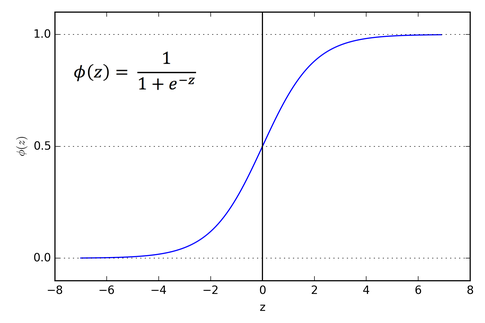
\includegraphics[width=0.38\textwidth]{sigmoid_logistic_regression.png}
\end{wrapfigure}
\vspace{6pt}

Instead what we do in logistic regression is $\hat{y}=\sigma(w^Tx+b)$, where $\sigma$ is the sigmoid function (shown in the diagram alongside, ignore the $\phi(z)$ notation). Defining $z=w^Tx+b$,
\begin{center}
$\boxed{\sigma(z)=\dfrac{1}{1+e^{-z}}}$
\end{center}
If $z$ is a large positive number, $e^{-z}\rightarrow 0$, $\therefore\sigma(z)\rightarrow 1$

If $z$ is a large negative number, $e^{-z}\rightarrow \infty$, $\therefore\sigma(z)\rightarrow 0$
\vspace{6pt}

We have now seen the logistic regression model in quite a bit of detail. However, to train the parameters $w$ and $b$, we need to define a cost function.
\subsection{Cost function in logistic regression}
To train the parameters of our logistic regression model, we have a training set of $m$ training examples. Given $\{(x^{(1)},y^{(1)}), (x^{(2)},y^{(2)}), \dots, (x^{(m)},y^{(m)})\}$, we want to find parameters $w$ and $b$ so that $\hat{y}^{(i)}\approx y^{(i)}$. To recap, $$\hat{y}^{(i)}=\sigma(z^{(i)})=\dfrac{1}{1+e^{-z^{(i)}}}\text{ where }z^{(i)}=w^Tx^{(i)}+b$$
Let us now see a loss/error function we can use to measure how well our algorithm is doing. One thing we could do (that, again, doesn't work) is define $\Lagr(\hat{y},y)=\dfrac{1}{2}(\hat{y}-y)^2$. In practice, this leads to the optimization becoming non-convex (i.e. we end up with multiple local optima), so gradient descent (discussed in the next section) may not find the global optimum.
\vspace{6pt}

Instead, we define a different loss function to get a convex optimization problem. 
$$\boxed{\Lagr(\hat{y},y)=-(y\log\hat{y}+(1-y)\log(1-\hat{y}))}$$
On first sight, it seems this function was conjured from thin air. Here's some intuition for why it makes sense. If we use a squared error, then we would want the squared error to be as small as possible. Similarly, we also want the above loss function to be as small as possible. Let's look at 2 cases: 
\begin{itemize}
	\item if $y=1$: $\Lagr(\hat{y},y)=-\log\hat{y}\implies$ $\log\hat{y}$ to be large $\implies$  $\hat{y}$ to be large
\end{itemize}
But since $\hat{y}$ is a sigmoid function, it is always $\leqslant 1$. Hence, if $y=1$, we want $\hat{y}$ to be as close to 1 as possible.
\begin{itemize}
	\item if $y=0$: $\Lagr(\hat{y},y)=-\log(1-\hat{y})\implies$ $(1-\log\hat{y})$ to be large $\implies \log\hat{y}$ to be small $\implies \hat{y}$ to be small
\end{itemize}
But $\hat{y}$ can never be smaller than 0. Hence, if $y=0$, we want $\hat{y}$ to be as close to 0 as possible. One may argue that there are many such functions which roughly satisfy the 2 conditions above. We will discuss later why we choose a loss function with this particular form.
\vspace{6pt}

Finally, the loss function above is designed with respect to a single training example, i.e. it measures how well our algorithm is doing on a single example. Now let us define the cost function, which measures how well our algorithm is doing on the entire training set.
\vspace{6pt}

The cost function $J$, which is applied to parameters $w$ \& $b$, is just the simple average of the loss function applied to each of the training examples.
$$\boxed{J(w,b)=\dfrac{1}{m}\sum_{i=1}^{m}\Lagr(\hat{y}^{(i)},y^{(i)})=-\dfrac{1}{m}\sum_{i=1}^{m}\left[y^{(i)}\log\hat{y}^{(i)}+(1-y^{(i)})\log(1-\hat{y}^{(i)})\right]}$$
Using this, we try to find parameters $w$ \& $b$ that minimize the overall costs function $J$. 
\subsection{Gradient descent}
Up till now, we've seen the logistic regression model, the loss and cost functions for the parameters of the algorithm. Let us now see how the gradient descent algorithm can be used to train the parameters $w$ \& $b$ on a training set. From the previous section, we have the cost function
$$J(w,b)=\dfrac{1}{m}\sum_{i=1}^{m}\Lagr(\hat{y}^{(i)},y^{(i)})=-\dfrac{1}{m}\sum_{i=1}^{m}\left[y^{(i)}\log\hat{y}^{(i)}+(1-y^{(i)})\log(1-\hat{y}^{(i)})\right]$$
We naturally want to find $w, b$ that minimize $J(w,b)$. We do this using what is known as the gradient descent algorithm. Here's an illustration of gradient descent.
\begin{wrapfigure}[10]{R}{0.4\textwidth}
\centering 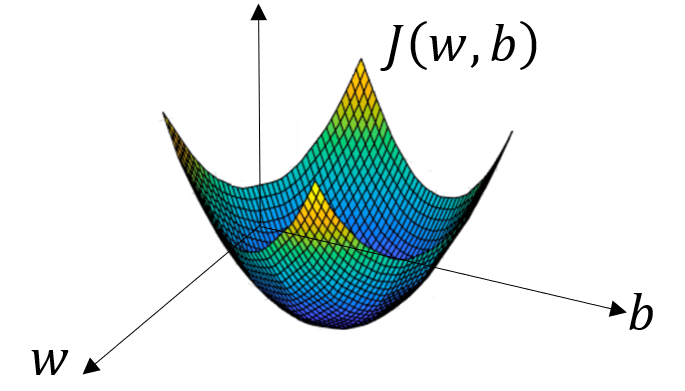
\includegraphics[width=0.38\textwidth]{gradient_descent.png}
\end{wrapfigure}
\vspace{6pt}

Note that, in practice, $w$ is of a much higher dimension, but for illustrative purposes let's assume it is a single real number. As seen, $J(w,b)$ has a single global optimum, and we want to find $w,b$ corresponding to this minimum.
\vspace{6pt}

To do this, we first initialize $w$ \& $b$ to some value (for convenience, we usually initialize them both to 0).
\vspace{6pt}

After this, what the gradient descent algorithm does is take a step in the steepest downhill direction. There can multiple iterations of the gradient descent cycle until the point the algorithm decides that it has reached the global optimum. 
\vspace{6pt}

This gives us a brief overview of how gradient descent works. Let's dive deeper into the details. Consider a one-dimensional plot with only $w$ as the parameter.
\begin{wrapfigure}[9]{L}{0.4\textwidth}
\centering 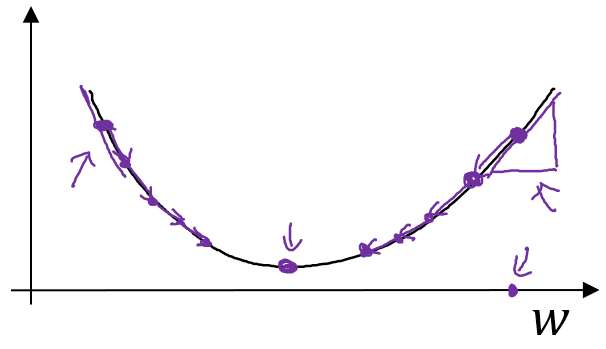
\includegraphics[width=0.38\textwidth]{1d_convex_plot.png}
\end{wrapfigure}
\vspace{6pt}

The gradient descent algorithm repeatedly carries out the following update until it converges to the global optimum value:
$$w\equiv w-\alpha\left(\frac{\text{d}J(w)}{\text{d}w}\right)$$
where $\alpha$ is the learning rate, which controls how big each step in the gradient descent is. 
\vspace{6pt}

No matter where we initialize the value of $w$, the gradient descent algorithm will always reach the global optimum at some point. 
\vspace{6pt}

Since we actually have a function $J$ in 2 parameters, the loop of gradient descent becomes as follows:
$$w\equiv w-\alpha\left(\frac{\partial J(w,b)}{\partial w}\right)\text{; } b\equiv b-\alpha\left(\frac{\partial J(w,b)}{\partial b}\right)$$
When we actually get down to coding such and algorithm, we will use the following (mathematically inconsistent) notation:
$$\text{d}w\equiv \frac{\partial J(w,b)}{\partial w} \text{; } \text{d}b\equiv \frac{\partial J(w,b)}{\partial b}\longrightarrow w\equiv w-\alpha\text{d}w; b\equiv b-\alpha\text{d}b$$ 
\subsection{Computation graph}
\textit{(This section is currently in the works. Expect it to be up typically within a week's time.)}

\hrulefill
\end{document}
